%-------------------------------------------------------------------------------
\section{Problem}\label{s:problem}
%-------------------------------------------------------------------------------

We find that Kubernetes violates the expectation of stable performance for high
QOS class pods: Guaranteed as well as Burstable pods see latency impacts from
load on other services. We track the issue down to Linux' \cgroups{}, and show
that its interface is not conducive to supporting the QOS guarantees outlined.

We use as a case study a small but realistic social network web application,
which we run using Kubernetes. To run other workloads alongside it, we use a
CPU-bound server for Guaranteed or Burstable, and an image resize job for the
BestEffort QOS class. In all cases, we run two pods, each requesting 2 cores, on
the same four cores.


\subsection{BestEffort pods impact Burstable and Guaranteed performance}

A key tenet of the QOS classes is that the lowest class, BestEffort, be
invisible to higher classes. BestEffort tasks need to be preempted as soon as a
higher class pod has anything to run. If this is correctly enforced, no amount
of load on a BestEffort pod should be able to affect the performance of a
Guaranteed or Burstable pod.


\begin{figure}[t]
    \centering
    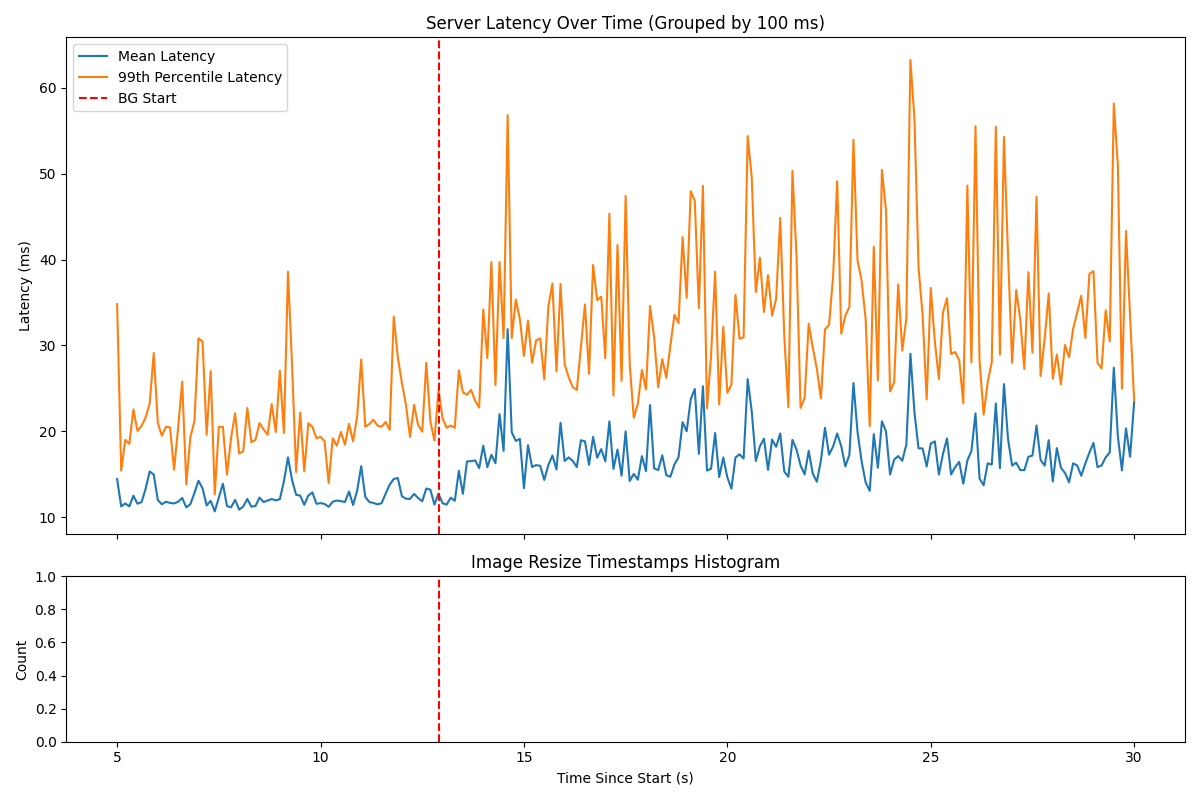
\includegraphics[width=\columnwidth]{graphs/kubernetes-unedited.png}
    \caption{Running a BestEffort affects the server's
    performance}\label{fig:kubernetes-unedited}
\end{figure}

However, we find that running a BestEffort job does in fact impact the
performance of higher class pods. \autoref{fig:kubernetes-unedited} shows the
result of running a best effort workload, using the BestEffort class, alongside
the web server, running as a Burstable pod. The top graph plots the end-to-end
latency of an endpoint that gets a users feed and applies a moderation; the
bottom graph shows the throughput of a best effort image resize job. After the
image resize job starts running, the mean response latency of the web
application jumps from $\sim$7ms to $\sim$15ms, and the 99th percentile latency
from $\sim$10ms to $\sim$25ms. The graph looks the same if the web server is
running as a Guaranteed pod. This clearly violates the goal that Guaranteed and
Burstable pods get access to reserved CPUs when they could use them.


\begin{figure}[t]
    \centering
    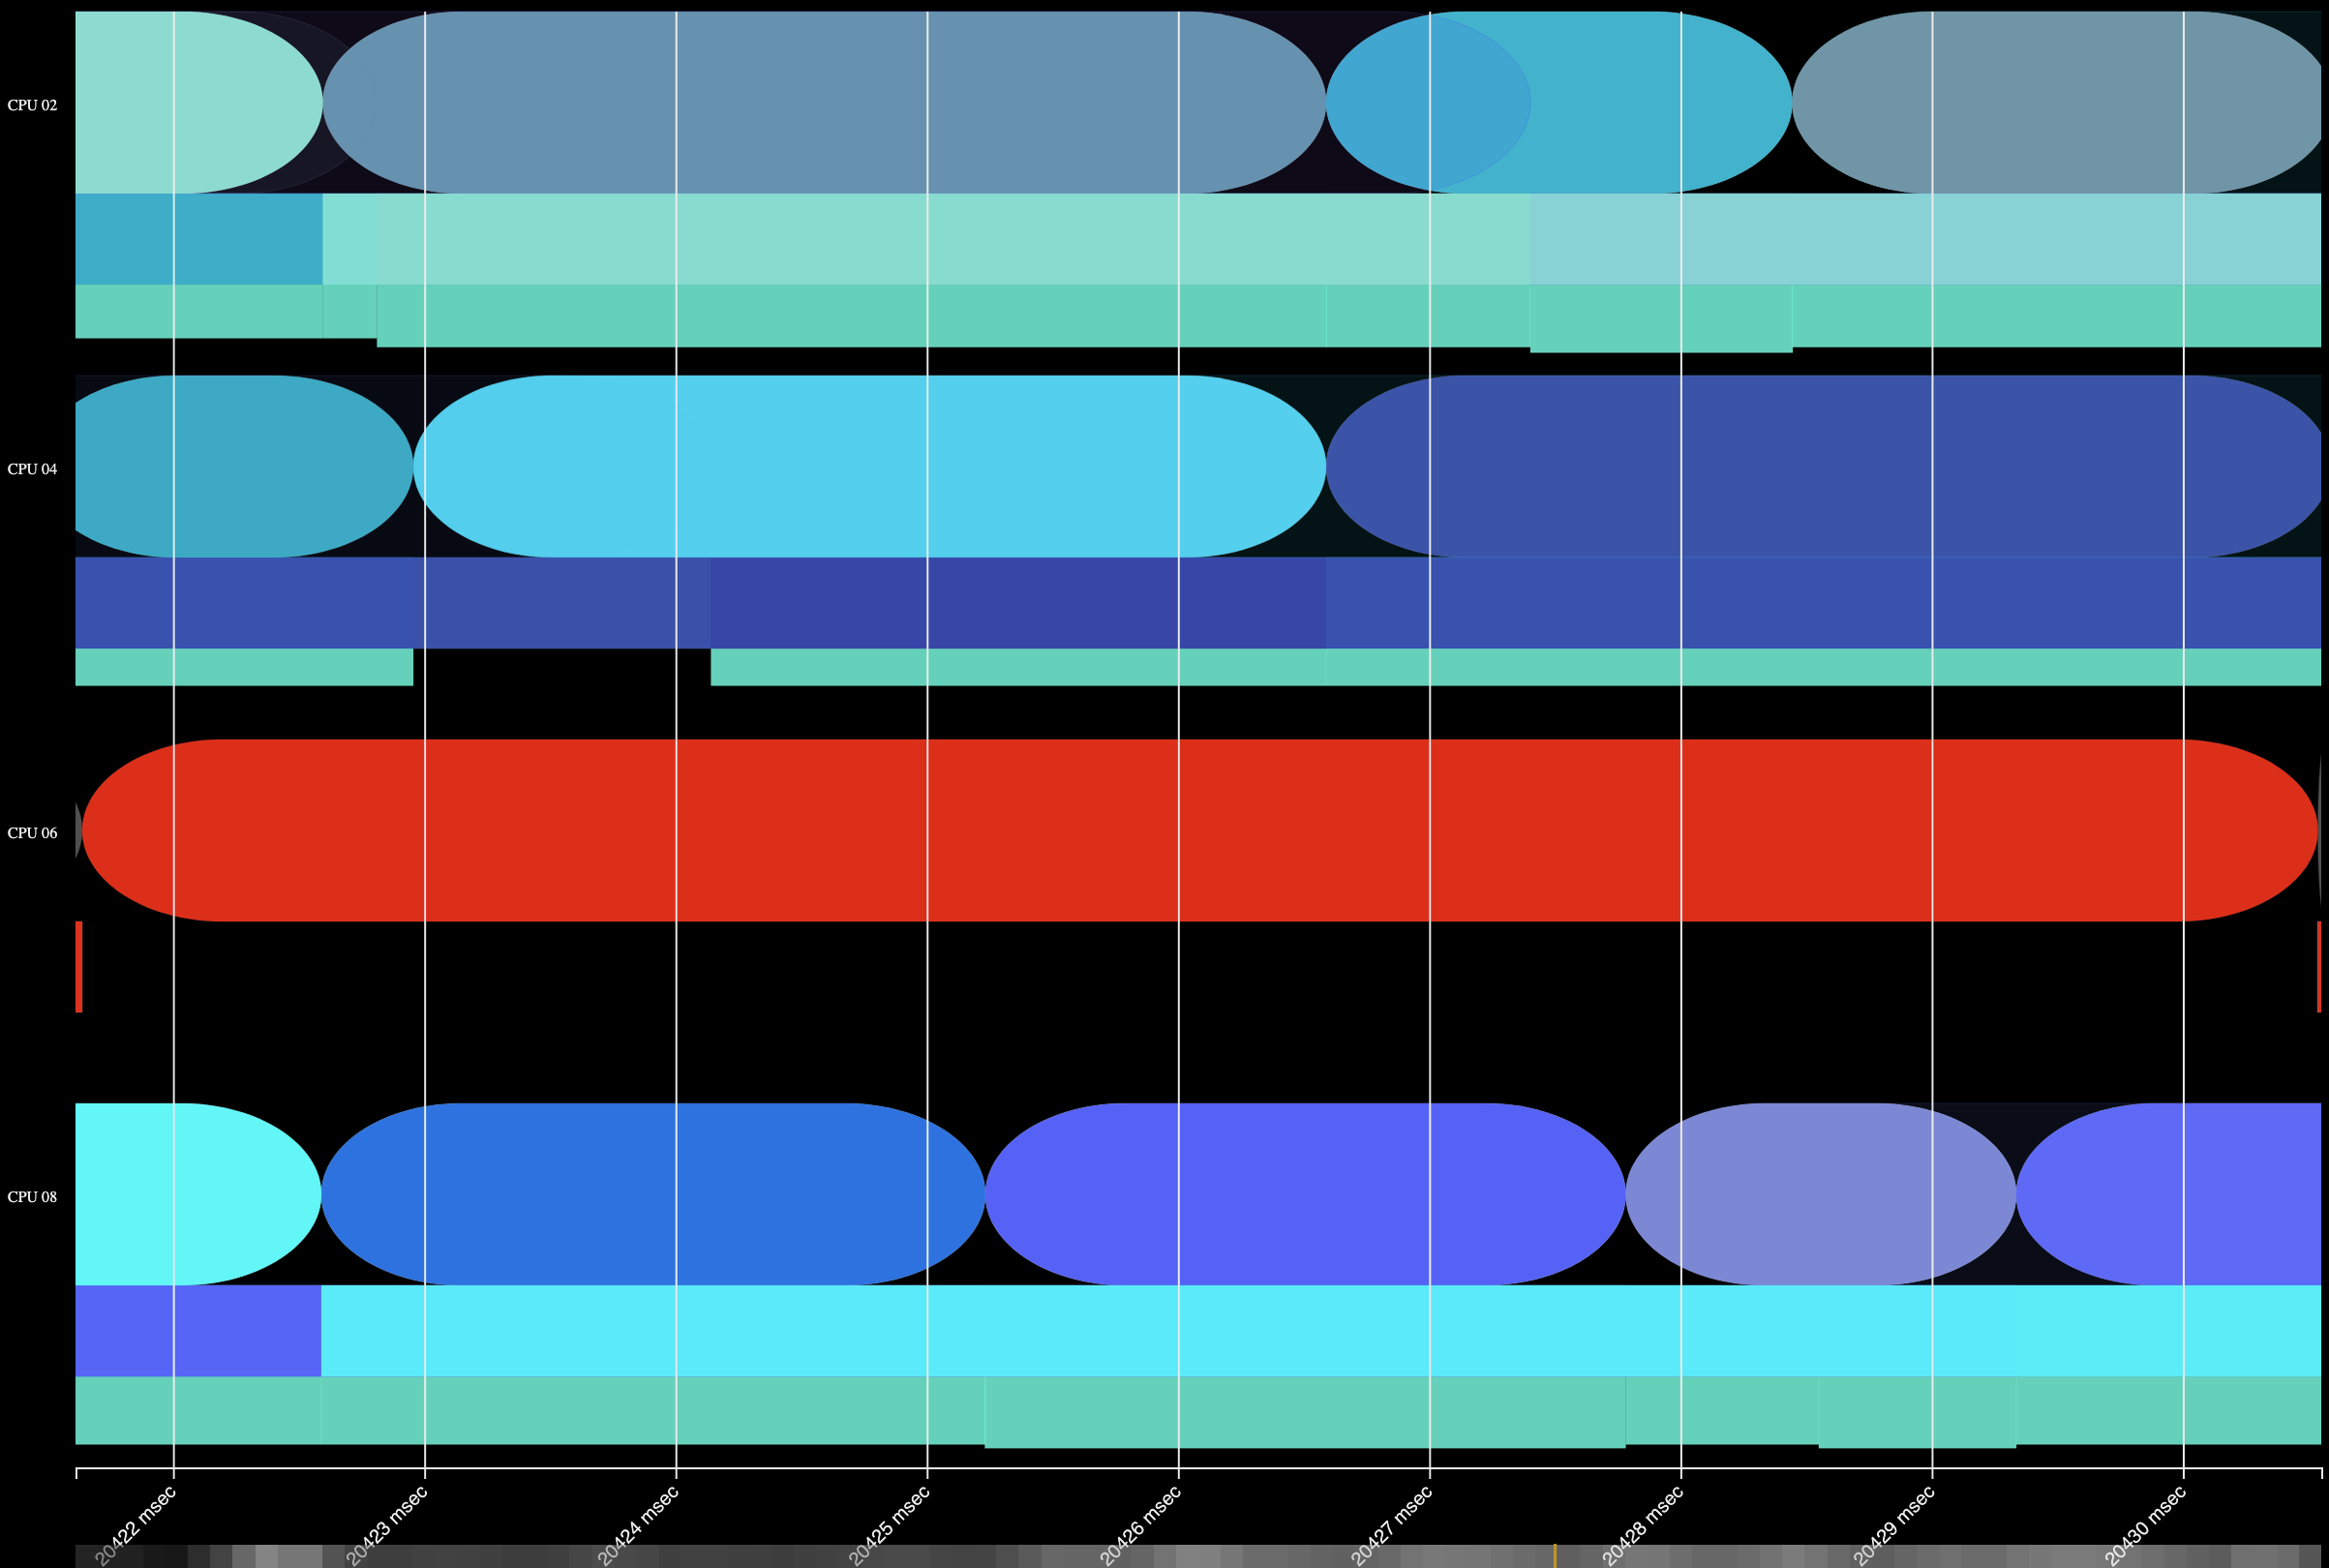
\includegraphics[width=\columnwidth]{graphs/schedviz-be-problem.png}
    \caption{Core 6 runs an image resize process, unaware that cores 2, 4, and 8
    all have runnable and queued server threads}\label{fig:schedviz-be-problem}
\end{figure}

To understand where the performance impact is coming from, we visualize the
trace of the experiment using schedviz~\cite{schedviz-tool}. What we find is
that frequently \textit{one core is running a best effort process, while threads
of processes with resource reservations are queued on another}.
\autoref{fig:schedviz-be-problem} shows an outtake from the trace. The process
running on each core is shown as an oval, and queued processes are shown as
rectangles below; the x-axis is time and the y-axis shows the 4 cores the
experiment is running on. We see that on one of the cores, the red process that
is running for the whole 10ms is a thread of the image resize job, while server
threads, shown in varying shades of blue, are queued on the other cores.

Understanding why this is happening requires understanding how Kubernetes
enforces the CPU isolation between pods. Kubernetes uses the \cgroups{} weight
interface to enforce pods' CPU requests: It makes sure that machines are never
oversubscribed on requested CPU, and then uses weights to split up the cores on
the machine.

Burstable and Guaranteed pods are given a weight that is calculated based on the
number of cores the machine has and how many CPUs the pod requested. For
instance, on a 56 core machine we found that a pod that requested 4 cores was
given a weight of 157, whereas one that request 2 CPUs was given a weight of 79.
Kubernetes uses the smallest weight possible, 1, to run BestEffort pods.

The key fact relevant here about \cgroups{} weight is that \textit{weights are a
local property}. Linux maintains a separate runqueue on each core, and within
each runqueue, Linux's scheduler works to maintain the correct ratio of received
CPU time at each scheduling; but Linux does not enforce the weight ratios across
cores.

The observed inversion happens then because the threading model of the server
interacts with the per-core runqueues. The server uses a pool of worker threads
(one per client). The number of threads that the server has is larger than the
number of cores, which means that each core has multiple server threads. It
occasionally occurs that all the current requests are on server threads that
happen to be on only three of the four available cores, which leaves one
runqeueue with only idle server worker threads. This leads to an inversion,
where the core that has no runnable high weight server threads and thus runs a
low weight image resize thread, even while other cores have queued high weight
processes.


\subsection{Pods with reservations affect each other's performance}

Another relevant promise of the QOS-class-based interface is that two pods with
reservations not affect each other. Because Kubernetes never oversubscribes on
requests, that means that every pod with a reservation should be able to get
access to the requested CPUs and use whenever they have enough load to. We would
then expect that no amount of load on a Burstable pod should affect another pod
with its own reservation, if the latter can service its load with the requested
amount of CPUs.


\begin{figure}[t]
    \centering
    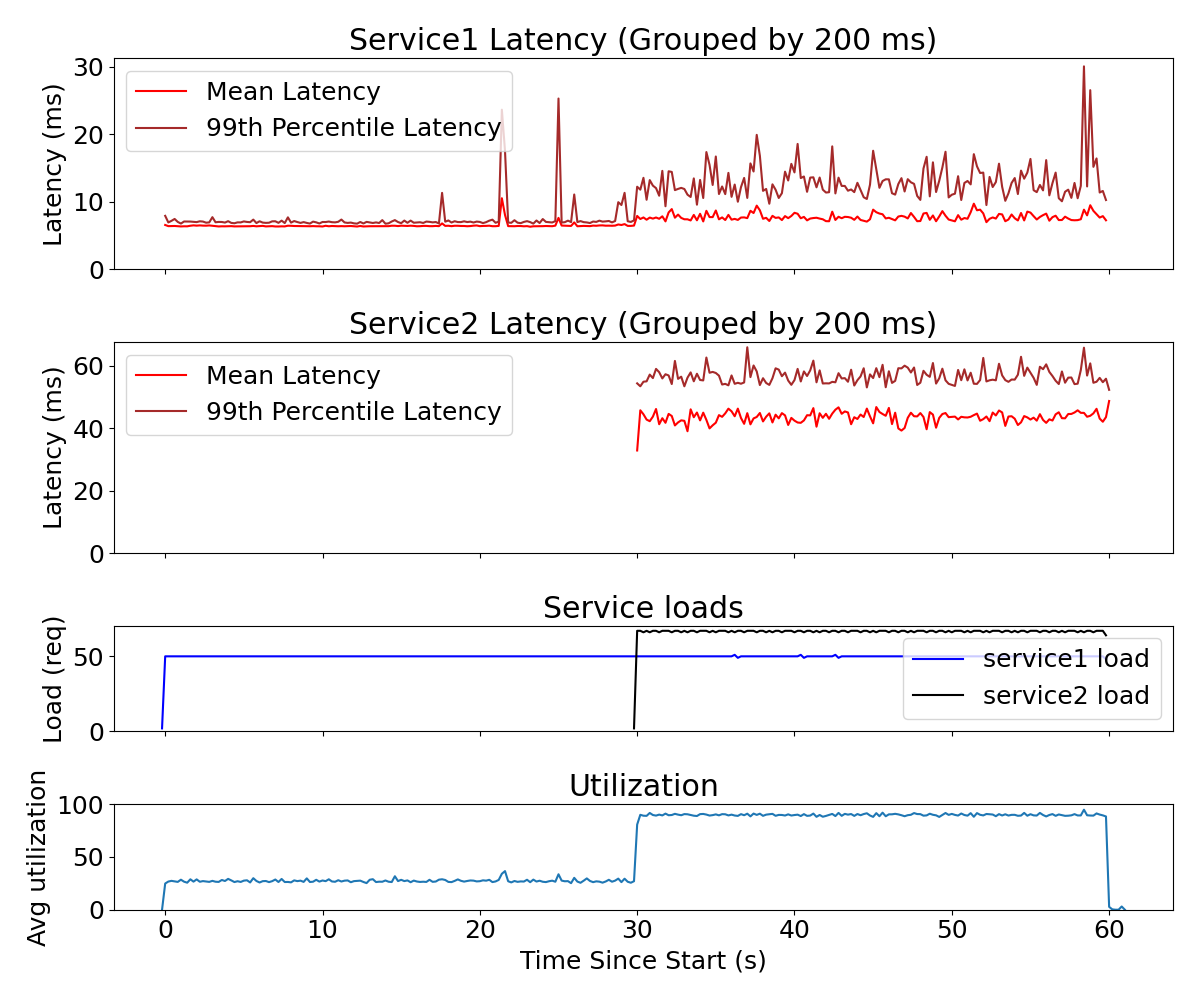
\includegraphics[width=\columnwidth]{graphs/kubernetes-lc-burst.png}
    \caption{In Kubernetes, running a Burstable server2 alongside the Guaranteed
    server1 affects server1's performance}\label{fig:kubernetes-lc-burst}
\end{figure}

To test this expectation, we run experiments using two servers: server1 runs the
same web server, and server2 is a simple CPU-bound server. 

\subsubsection{Burstable pods affect Guaranteed pods}

We run the web server in the Guaranteed class, and server2 in the Burstable
class. Surprisingly, we see a significant latency impact under high load.
\autoref{fig:kubernetes-lc-burst} shows the web server's latency and the overall
utilization, before and after starting load on server2. We see that average
latency jumps from $\sim$6ms to $\sim$9.5, and the 99th pctile from 7ms to 22.

\begin{figure}[t]
    \centering
    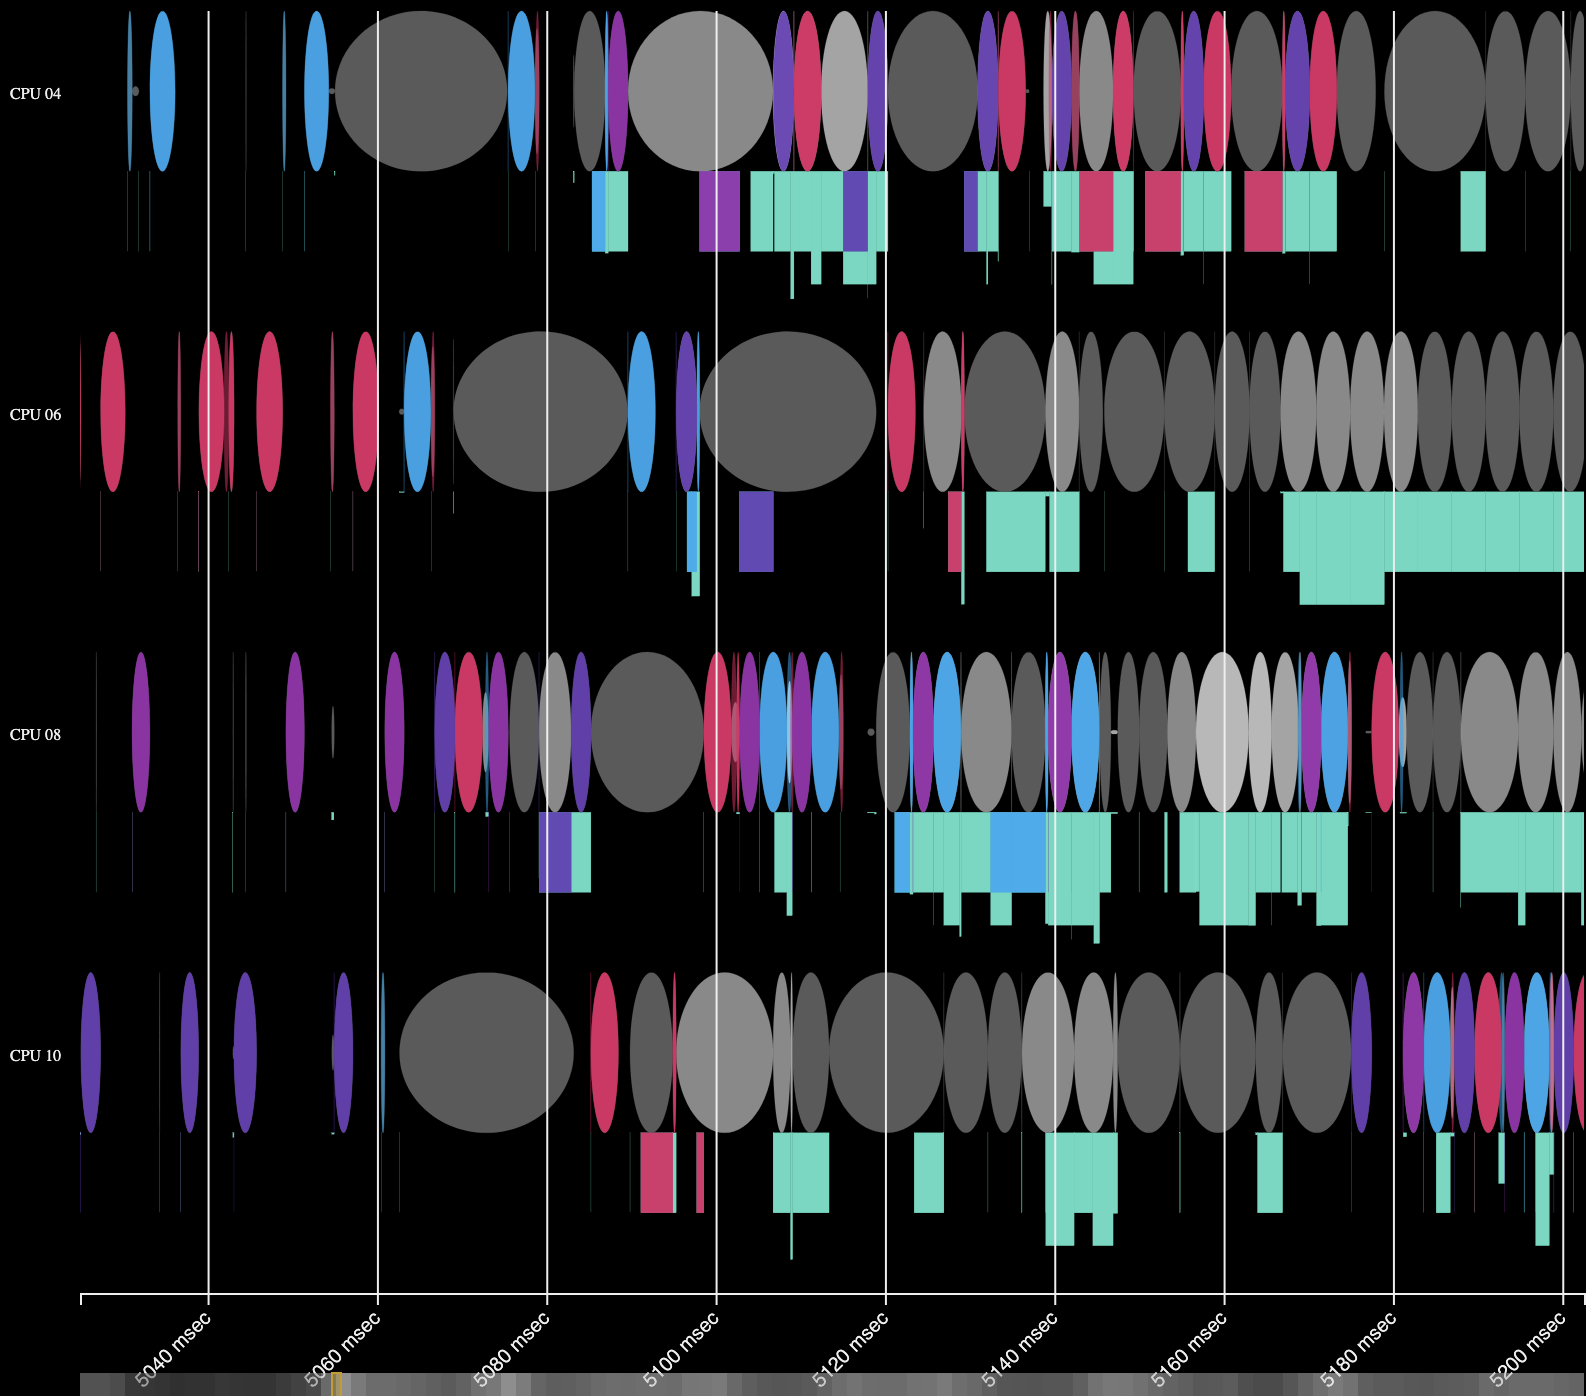
\includegraphics[width=\columnwidth]{graphs/schedviz-lc-burst-problem.png}
    \caption{When server1 is running alone, it has all the cores to itself, but
    after server2 starts it gets only half of whatever core it runs on, even if
    it isn't using all the cores available and server2 is running uncontended on
    the other cores}\label{fig:schedviz-lc-burst-problem}
\end{figure}

\autoref{fig:schedviz-lc-burst-problem} shows an outtake from the trace of the
experiment. Threads of server1 are colored in, threads are serer2 are shown in
shades of grey. On the very left of the trace, server1 can run uncontended on
any core when requests come in. Then server2 starts, and has a high load and
thus immediately starts running on all four cores, because it is Burstable. When
a request from server1 comes in, the thread processing that request has to share
the core equally with threads from server2, or other server1 threads, while
while server2 gets other cores all to itself.

This means that Burstable pods have a performance impact on Guaranteed ones
because both share cores where they both have threads as equals, irrespective of
who is running how much on other cores. In particular, server1 has less load and
thus less runnable threads. However, on the few cores where its threads are
runnable, it will have to share that core equally; even while the server with
higher load runs uncontended on other cores. We conclude that the issue boils
down to the locality of weights again: if the core with both servers' threads
knew server2 had other cores all to itself it could compensate, but it doesn't
know, so it treats both equally.


\subsubsection{Guaranteed pods affect other Guaranteed pods}

One might think that two Guaranteed pods avoid this issue: because they are both
limited to the amount of CPUs they requested, one can't burst and be a contender
on many more cores than the other.

\begin{figure}[t]
    \centering
    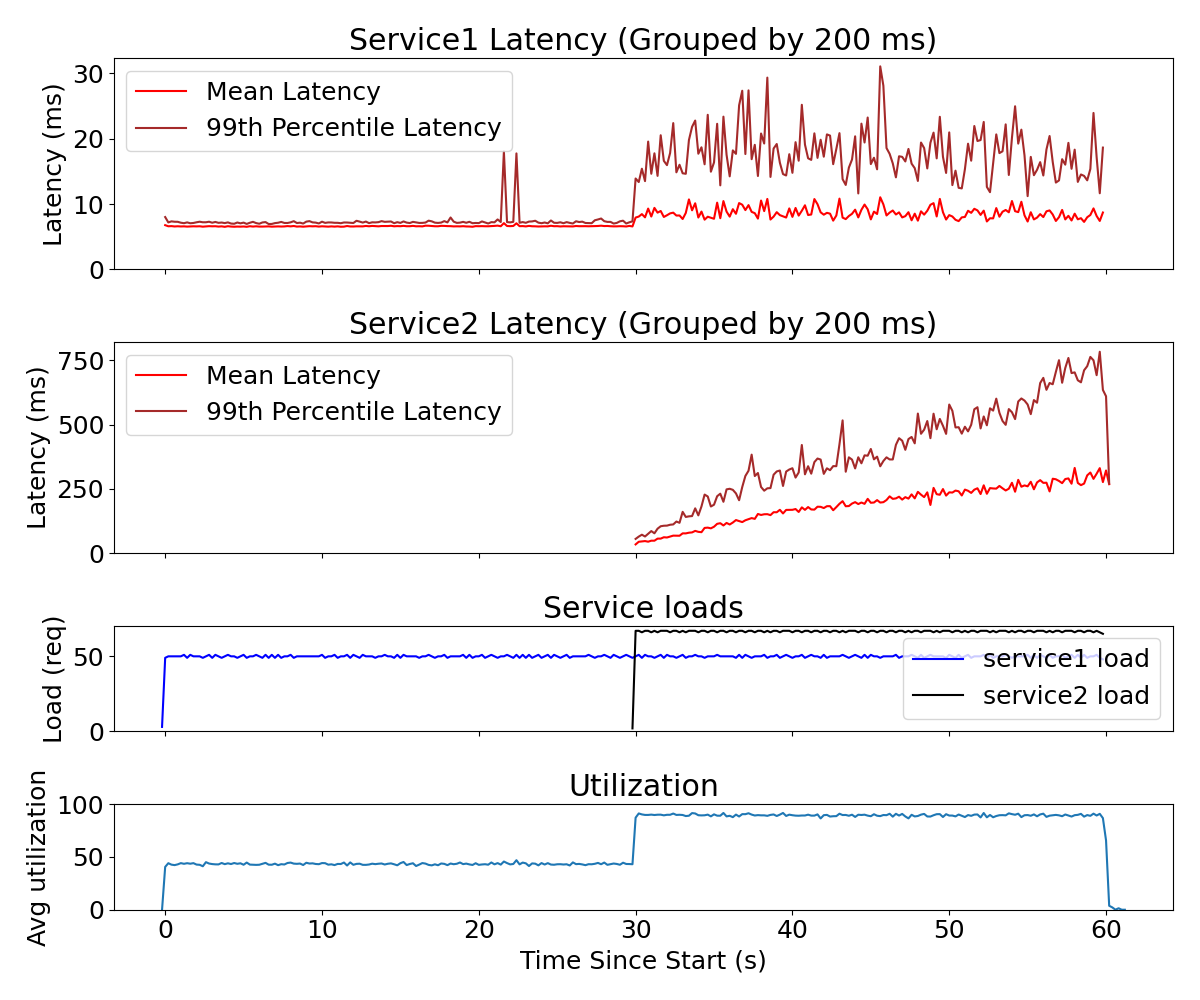
\includegraphics[width=\columnwidth]{graphs/kubernetes-lc-guar.png}
    \caption{In Kubernetes, running a Guaranteed server2 alongside the
    Guaranteed server1 affects server1's
    performance}\label{fig:kubernetes-lc-guar}
\end{figure}

However, we find that even a Guaranteed pod can impact anothers performance. We
run the same two servers, both now in the Guaranteed class.
\autoref{fig:kubernetes-lc-guar} shows the result: average latency jumps up by
$\sim$4ms, and 99th pctile by $\sim$ 20ms.

The reason this problem happens is related to how Kubernetes uses \cgroups{} to
enforce limits on pods. Kubernetes uses cpu.max to do so, but the interface to
\cgroups{} cpu.max is different from that of Kuberentes' milliCPUs: \cgroups{}
asks instead for a runtime $r$ and a period $p$, and ensures that the group
never gets more than $r$ CPU time per $p$ time period. Because multiple threads
can run at the same time, it is possible that $r>p$.

\begin{figure}[t]
    \centering
    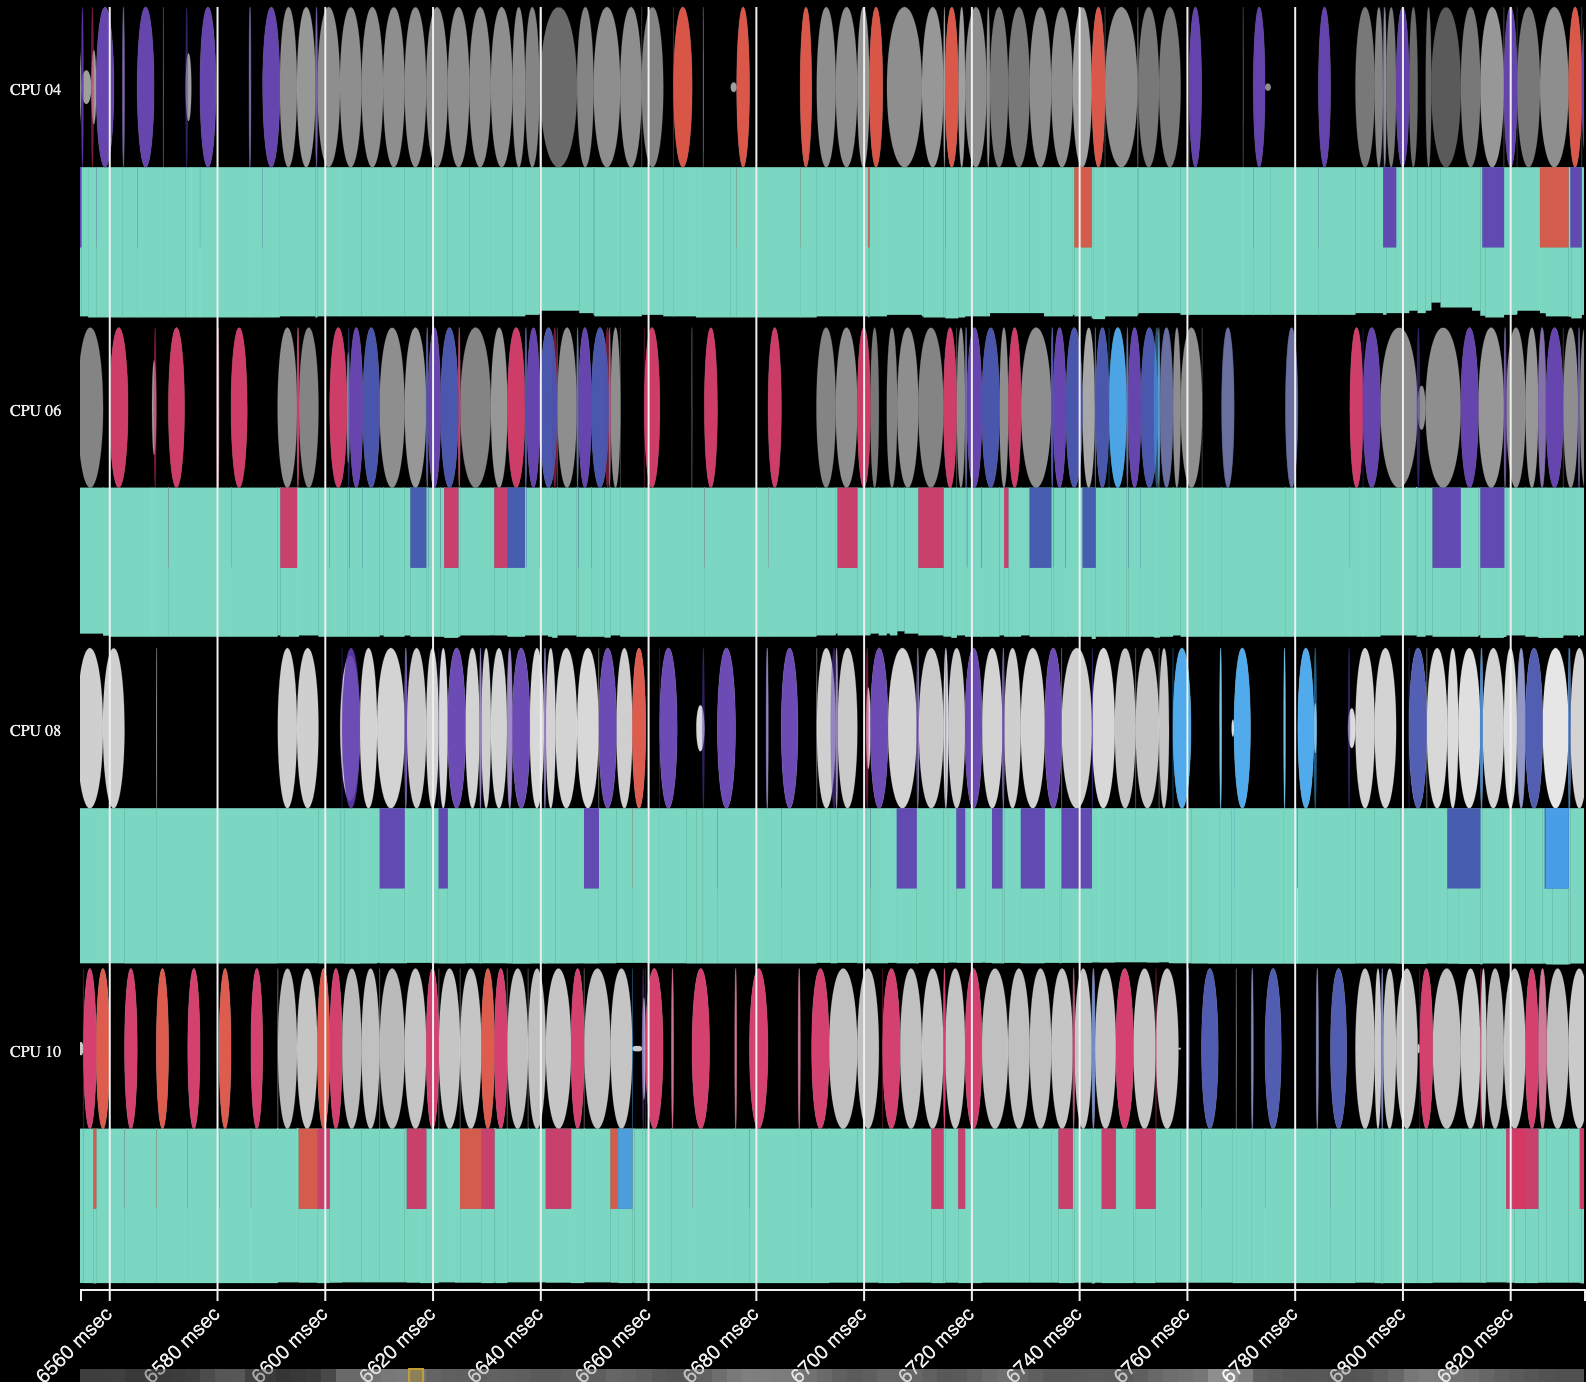
\includegraphics[width=\columnwidth]{graphs/schedviz-lc-guar-problem.png}
    \caption{When server1 is running alone, it has all the cores to itself, but
    after server2 starts it gets only half of whatever core it runs on, even if
    that is a fraction of the cores available and server2 is running uncontended
    on the other cores}\label{fig:schedviz-lc-guar-problem}
\end{figure}

Enforcing a limit of 2 vCPUs is different than enforcing that a group only get
2ms of CPU time every 1ms. If a pod is restricted to 2 vCPUs, then it can run up
to two things at the same time, and thus use only up to two cores. However, if a
group is limited to 2ms every 1ms, it could also fill its quota by running four
things on four cores for half a ms. In the time when one group is running on all
four cores, Kubernetes relies on weights to separate the two, which can lead to
significant delays for other services, as we saw.
\autoref{fig:schedviz-lc-guar-problem} shows this happening in a trace from the
experiment from \autoref{fig:kubernetes-lc-guar}. We can see the phases of
server2 threads, which are shown in grey: they run for a while on all four
cores, disrupting the colorful server1 threads, before being throttled, during
which time server1 threads can run uninterrupted and otherwise the cores lie
idle.

\hmng{I should add a note somewhere that lots of people caution against using
limits for exactly this reason, and cite the reddit articles/presentations I
found}

\subsection{Things that you might think fix it, but don't}

\subsubsection{Load balancing}

Linux performs periodic load balancing, where it works to equalize the weight
across different cores. However, load balancing runs significiantly less
frequently than scheduling does, at least during high load. How often load
balancing runs in general is a complicated number that is dependent on how close
the two cores are in the CPU architecture hierarchy, as well as how loaded the
machine is. This means that in the context of a stable set of long-running
processes, load balancing can ensure that no two cores have wildly different
total weights and thus that the time each thread gets on each core reflects the
time it should get overall. However, in the context of short-lived request
processing with a constantly changing set of runnable worker threads, load
balancing is not enough.

\begin{figure}[t]
    \centering
    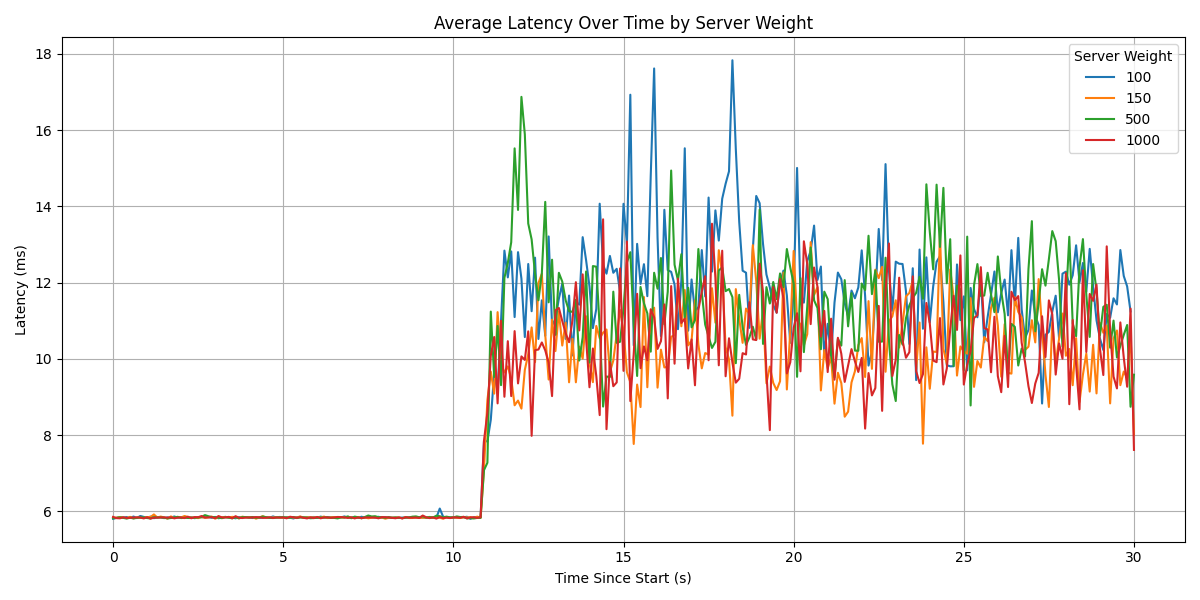
\includegraphics[width=\columnwidth]{graphs/srv-bg-weight-cmp-low.png}
    \caption{Changing the weight of the server beyond 100 has little impact on
    how much the weight 1 best effort task interferes with
    it}\label{fig:srv-bg-weight-cmp}
\end{figure}

\subsubsection{Bigger weight splits}

As we saw in our experiment, Kubernetes uses a weight split of around 79:1,
whereas Linux supports weights in the range of [10000,1]. We show that a larger
weight split does not fix the problem. We demonstrate this with a
microbenchmark, which runs a simple CPU-bound server with a pool of worker
threads. We run an open-loop client on a remote machine, and then start two best
effort workloads doing image resizing. We put the server and the image resize
job each in their own \cgroups{} group, and pin them to the same set of four
cores. The image resize job always has weight 1, and we vary the weight of the
server. \autoref{fig:srv-bg-weight-cmp} shows that using a bigger weight split
has no impact on the latency impact of the best effort task. For all the
weights, at a $\sim$85\% baseline utilization of the server the server's mean
latencies spike up from steady at around 6ms to $\sim$15ms, and much higher for
99th percentile latencies. At a baseline utilization of 95\%, those numbers
increase to up to 40ms for the the mean latency, and 80ms for the tail.

\subsection{Summary}

From this section we conclude that the reason why Kubernetes fails to enforce
reservations as expected is \cgroups{}, and they way Kubernetes uses its
interface. There are two main ways \cgroups{} fails to provide Kubernetes with
an interface conducive to enforcing reservations.

\textit{\cgroups{} enforces weight splits locally.} Linux uses per-CPU
runqueues, and only enforces weights on a per-runqueues basis. This means that
temporary but frequent imbalances can lead to frequent priority inversion. The
result is that a pod with a reservation is forced to run and queue on fewer
cores than it reserved.

\textit{\cgroups{} max interface is unintuitive and enforces a meaningfully
different interface than a reservation.} Because the cpu.max interface is based
on a runtime quota that is bulk-renewed, groups can essentially still burst,
just for a limited amount of time. This creates a cyclic dynamic of bursting and
affecting other pods, and then being throttled.



